\documentclass[12pt]{ucthesis}

\usepackage{etex}
\usepackage[morefloats=125]{morefloats}
\usepackage[hyphens]{url}
\usepackage[caption=false]{subfig}
\usepackage{graphicx}
\usepackage{tabularx}
\usepackage{amssymb}
\usepackage{amsmath}
\usepackage[letterpaper]{geometry}
\usepackage[overload]{textcase}
\usepackage{color}
\usepackage[nonumberlist,toc]{glossaries}
\usepackage{wrapfig}
\usepackage{longtable}
\usepackage{morefloats}
\usepackage{float}
\usepackage{listings}
\usepackage{makecell}
\usepackage{appendix}
\usepackage[]{algorithm2e}
\usepackage{titlesec}
\usepackage[breaklinks=true,hidelinks,pdfusetitle]{hyperref}
\usepackage{cleveref}
\usepackage{ifthen}

\setcounter{secnumdepth}{3}
\setcounter{tocdepth}{3}

% Added to avoid windows and orphans
\usepackage[all]{nowidow}
% Added to fix spacing between footnote entries
\usepackage{setspace}
\newlength{\myfootnotesep}
\setlength{\myfootnotesep}{\baselineskip}
\addtolength{\myfootnotesep}{-\footnotesep}
\setlength{\footnotesep}{\myfootnotesep} % set spacing between footnotes

\makeindex

% Shrink the size of headers
\titleformat{\chapter}[display]
        {\normalfont\normalsize\centering}
        {\ifthenelse{\equal{\thechapter}{A}}{APPENDICES\\[4.3ex]}{}\chaptertitlename\ \thechapter}
        {0pt}{\normalsize\uppercase}
\titlespacing*{\chapter}{0pt}{-20pt}{4.3ex plus .2ex}


\titleformat*{\section}{\normalsize\bfseries}
\titleformat*{\subsection}{\small\bfseries}
\titleformat*{\subsubsection}{\small\bfseries}
\titleformat*{\paragraph}{\small\bfseries}
\titleformat*{\subparagraph}{\small\bfseries}

\bibliographystyle{abbrv}

% Make \tindent indent pages if you have no paragraph indent
\newlength\tindent
\setlength{\tindent}{\parindent}
\setlength{\parindent}{0.in} \setlength{\parskip}{1.em}
\renewcommand{\indent}{\hspace*{\tindent}}
% Otherwise, comment out the above and uncomment this for default indentation on each paragraph
%\setlength{\parindent}{0.25in} \setlength{\parskip}{6pt}

\geometry{verbose,nohead,tmargin=1in,bmargin=1in,lmargin=1.5in,rmargin=1in}

% Different font in captions (single-spaced, bold) ------------
\newcommand{\captionfonts}{\small\bf\ssp}

\newcommand{\mycaption}[2]{\caption[#1 --- #2]{#1 --- #2}}

\makeatletter  % Allow the use of @ in command names
\long\def\@makecaption#1#2{%
  \vskip\abovecaptionskip
  \sbox\@tempboxa{{\captionfonts #1: #2}}%
  \ifdim \wd\@tempboxa >\hsize
    {\captionfonts #1: #2\par}
  \else
    \hbox to\hsize{\hfil\box\@tempboxa\hfil}%
  \fi
  \vskip\belowcaptionskip}
\makeatother   % Cancel the effect of \makeatletter
% ---------------------------------------

% Define Appendix refs
\crefname{app}{appendix}{appendices}
\Crefname{app}{Appendix}{Appendices}

% Add Figures folder to the graphics path
\graphicspath{{Figures/}{figures/}}

% Options for hyperref
\hypersetup{
    bookmarksnumbered=true,
    bookmarksopen=false,
    bookmarksopenlevel=0,
    colorlinks=false,
    pdfstartview=Fit,
    pdfborder={0 0 0},
}

\newcounter{qcounter}
\providecommand{\keywords}[1]{\textbf{\textit{Keywords:}} #1}


\begin{document}

% Declarations for Front Matter
\title{A Homegrown DSMC-PIC Model for Electric Propulsion Plumes}
\author{Dominic Lunde}
\degreemonth{June} \degreeyear{2019} \degree{Master of Science}
\defensemonth{May} \defenseyear{2019}
\numberofmembers{4}
   \chair{Amelia Greig, Ph.D. \linebreak Professor of Aerospace Engineering}
   \othermemberA{David Marshall, Ph.D. \linebreak Department Chair, Aerospace Engineering}
   \othermemberB{Kim Shollenberger, Ph.D. \linebreak Professor of Mechanical Engineering}
   \othermemberC{Robert Martin \linebreak Computational Scientist, Air Force Research Laboratory}
\field{Aerospace Engineering} \campus{San Luis Obispo}
\copyrightyears{seven}


\maketitle

\begin{frontmatter}

% Custom made for Cal Poly (by Mark Barry, modified by Andrew Tsui).
\copyrightpage

% Custom made for Cal Poly (by Andrew Tsui).
\committeemembershippage

\begin{abstract}
Powering spacecraft with electric propulsion is becoming more common, especially in CubeSat-class satellites. On account of the risk spacecraft interactions, it is important to have robust analysis and modeling tools of electric propulsion engines, particularly of the plasma plume. The Navier-Stokes equations used in classic continuum computational fluid dynamics do not apply to the rarefied plasma, and therefore another method must be used to model the flow. A good solution is to use the Direct Simulation Monte Carlo (DSMC) method, which uses a combination of particle modeling and statistical methods for modeling the simulated molecules. 

A DSMC simulation known as SINATRA has been developed with the goal to model electric propulsion plumes. SINATRA uses an octree mesh, written in C++, and is designed to be expanded by further research. SINATRA has been initially validated through several tests and comparisons to theoretical data and other DSMC models. Multiple molecular model and collision schemes were also tested for validity, accuracy, and speed. This thesis examines expanding the functionality of SINATRA to simulate charged particles and make SINATRA a DSMC-PIC hybrid. The electric potential is calculated through a 7 point 3D stencil on the mesh nodes and solved with a Gauss-Seidel solver. It is validated through test cases of charged particles to demonstrate the accuracy and capabilities of the model. It includes additional features to simplify further research including  a comprehensive User Manual, industry version control, simple text file inputs, GUI control, and simple parallelism of the simulation. 

%[[The first paragraph of the abstract is good. The second one is more of a "methods" section. I want results! What did you find? 

%I should be able to read an abstract and understand the premise of an experiment (not the details) and the results. ]]
\end{abstract}

\begin{acknowledgements}
\noindent
Thanks to:
\begin{itemize}
    \item Dr. Amelia Greig  
    \item[] Thank you for being my thesis advisor, for being my teacher, for introducing me to the world of Aerospace Engineering, for trusting me in this thesis, for sending me to Japan, and for pushing me so hard that I finally felt like a Rocket Scientist.
    \item Dad   
    \item[] Thank you for always being there for me, for camping at the KOA and showing me Cal Poly, for always supporting my life decisions, for all the fall down hugs, and for giving me the slight nudges I need to get work done. Thank you also to the rest of my family. Mom, thank you for always being there for me, and being willing to put me first if I need it. Janelle, thank you for being a constant source of inspiration to me in aspirations, faith, and enjoyment of life. Shawn, thank you for being stoked about the things that I am stoked about, including me in your life, and for pushing me along on this thesis. Nico, thank you for showing me all the love I would ever need. Also, thank you Emily for being my Cal Poly buddy and for editing this thesis.
    \item Mac   
    \item[] Thank you for dealing with scatterbrained Dom, for becoming my friend, for being such a hard worker, and for inspiring me to see the world.
    \item[] 
    \item[] 
    \item David   
    \item[] Thank you for understanding that I was still catching on to the whole Engineering thing during the beginning of thesis, for working so dang hard on this project, and for writing a good thesis so I understand what's happening. 
    \item  Dr. Graham Doig   
    \item[] Thank you for being an incredible boss, for supporting me even though you didn't really know me, for teaching amazing CFD and wind tunnel courses so I would have half an idea how to deal with fluids for this thesis, and for teaching through doing.
    \item PROVE team   
    \item[] Thank you for being a family away from home, for having dreams that are way up in the clouds, for giving Dawn your all, and for trusting me with her. Thank you Will for showing me how incredibly a boss can also be a friend. Thank you Thomas and Dave for inspiring me to work hard and dream big. Thank you Kirwan for being my not quite identical twin and for always getting fired up for me. Thank you Natalia for your complete and total love for your friends.
    \item Joe House   
    \item[] Thank you for being my family away from home and dealing with your teenage kid Dom learning how to live with peers. Julia, for always having an open ear. James, for always having an open and strong heart. Jess, for taking care of me especially during stitches. Nico, for having such passion for so many things and sharing it with us. Luke, for being so caring and loving to me, and genuinely wanting to know all about my life. Garrett, what are the odds you write one of these? Also thank you to the rest of my Newman community, you made me feel safe.
    \item Aero Grad   
    \item[] Thank you to the Aero department and especially the grad students for accepting a physics major into the fold and teaching me your ways. Thank you Brandon for mentoring me and having such a calm and understanding presence as a teacher. Thank you Harrison, Jake, and Matt for being my Aero older brothers. Thank you Daniel for being an awesome friend, and for all those late night rides home. Thank you Lucas for editing this thesis.
    \item SLOBS  
    \item[] Thank you SLOBS for being my bros. Thank you for pushing me every practice. Thank you for laughing with me, losing with me, bidding with me, and catching my hucks. Thank you Johnny for being a true friend with a heart of gold.
    \item Cho-lab  
    \item[] Thank you Cho-lab for making my stay in Japan one that changed how I view others for the good. Thank you for welcoming me with open arms and dealing with my loud American self. Thank you Takeshi for taking me under your wing but also allowing me to teach you as well. Thank you Hind for being my ride or die friend. Thank you Mark for investing in me as a person. Thank you Victor for coding support and for being genuinely interested and invested in me.
    \item Michele Da Silva  
    \item[] Thank you Mickey for always being a super fan of me. From the hours of frisbee nerd talk, hundreds of homework problems you helped me through, and for being a rock of a friend. I can't wait to see how you change the world next. 
    \item Andrew Guenther   
    \item[] Thank you for uploading this Latex template
\end{itemize}

\end{acknowledgements}

\tableofcontents

\listoftables

\listoffigures

% Add CHAPTER into table of contents.
\addtocontents{toc}{%
   \noindent CHAPTER
}

\end{frontmatter}

\pagestyle{plain}

\renewcommand{\baselinestretch}{1.66}

\chapter{Introduction}
\section{Motivation}
There are many methods to create something new. They all begin with an idea which needs realization. The path to realization in some cases can involve simply building the final project. However, with Aerospace Engineering that is not the case. To achieve the end goal much planning is needed. A idea is formed, the feasibility is researched, it is designed, and then built. With many Aerospace projects, designing a cutting edge project requires accurate physical modeling in order confirm the feasibility of the design and examine the effects of iterations. Therefore, the field of Aerospace simulation and modeling is a large and extensive field. It is one which is constantly changing and expanding as computing power becomes exponentially stronger. The boom in computing power has opened the door to this thesis. \par

\indent A large part of Aerospace research takes place within low density states of matter. Atmospheric reentry of spacecraft, objects in Low Earth Orbit, planes flying at extremely high altitudes, and interactions with plasma all operate within in relativly low density. 
% knudsten number

\subsection{Overarching Goal}
This thesis is one project in a planned series of projects. The goal is to have a Cal Poly homegrown simulation which can simulate an entire electric thruster. This is a task which has not yet been accomplished in manner which is reasonable for university researchers to use. A simulation of a full electric thruster requires a fluid based simulation for the gas inside the thruster and then a rarefied gas code for the exhaust plume. There aren't codes which have been built as one simulation, instead researcher attempt to join a fluid code and rarefied gas code together. This is where Cal Poly's Aerospace department is unique. A fluid code and a rarefied gas code are being developed from the ground up with a focus on the similarities. The early developers and advisors work together to build these codes to be compatible from the beginning. \par

\indent This thesis is the third project of the SINATRA code which will be able to simulate the thruster's plasma exhaust plume. The first three developers worked together in a staggered capacity to build SINATRA up to a working DSMC-PIC code. The first, David Galvez, developed the base framework and kinematics \cite{Galvez2018a}. Next Robert Alliston built up the collisions and particle models cite{Mac's Thesis}. This thesis adds charged particle simulation to SINATRA. At the same time as this thesis, Anthony Gay is building the fluid side simulation. Intentionally many things will be common between the codes. They are both written in C++ and are class based. They share the same process control items including the execution style, distribution method, and the other systems engineering items shown in Chapter \ref{chap:systems}. They share the same mesh type, input class, and other items to help them work together as one simulation. It is slated for future work for a project which takes both simulations and builds the interaction system to connect them across each timestep. 



% cite no full thruster code
% Cite macs thesis when it comes in


\chapter{Systems Engineering}
\label{chap:systems}
\section{Documentation}
In order for SINATRA to be used by other users and developer the code must be well documented. It is important to have systems of documentation in place for all of the different levels of instructions, guidelines, comments, and information. Those can be broken into two sections; for the user and for the developer. These systems must be simple, reliable, clear, and resilient. The goal is for the code to be easy to distribute, simple to learn as much as needed about how it works for that specific new purpose, and for the changes, bugs and suggestions to be centralized.
\subsection{GitHub}
The system chosen to organize and host SINATRA for developers is GitHub. It is a online file storage, syncing, and collaboration work space for developing code bases. It is easy to use, popular and therefore support for using it is strong, and it is very powerful. SINATRA is housed on GitHub by the author and is shared with Dr. Greig and Dr. Marshall. On account of the code's license the repository is private and developers can get access by contacting the Aerospace Department at Cal Poly, SLO. \par
\indent GitHub has three major features used in SINATRA; the commits system, the branches system, and the ReadME files. The commits system is a method of allowing multiple developers to work on the same code base without breaking the other developers builds. Each developer works on the code on their local machines. Once they have a stable addition to SINATRA, they commit it to GitHub. Whenever other users are working, they can pull those changes on to their local machine and developing moves along smoothly. It does require communication between the developers to ensure they aren't working on the same lines of code and creating different outcomes. This commit structure also allows the code base to be version controlled, which helps with mistakes and following the change logs. \par


\begin{figure}
\includegraphics[width=.95\textwidth]{branching.png}
\centering
\caption{Example of GitHub workflow}
\label{fig:github}
\end{figure}


\indent Another feature utilized during the development of SINATRA was the branches feature. This feature allowed a user to create a separate branch of the code base. They would use this to develop a large new section of code where they wanted the features and security of GitHub, but didn't want to clutter the teams main code with testing and validation edits. Once the branch becomes stable and ready to be released into the master branch, they can be merged through a pull request. The new features would then be available in the master branch for more development. This allows developers to command their own section of the code, update and test, and then make it available to the other developers to work with. This ensures a constant work flow where multiple developers can work on different features and not have to worry about whether their testing and tinkering will hinder others work on the master branch. In this way the development continues without bottlenecks and constant communication between the developers. \par
\indent The final feature used in GitHub was the ReadME files. These files are automatically displayed by GitHub's system when you enter the directory. This allows the developers to convey how that directory fits into the code base, and specifics on the files in the directory, and instructions on how to use the directory. The author has outfitted all of SINATRA's directories with ReadME files. These features were the reason that the author choose GitHub to host SINATRA and they were utilized during development in order to allow efficient and clear code creation. 

\begin{figure}
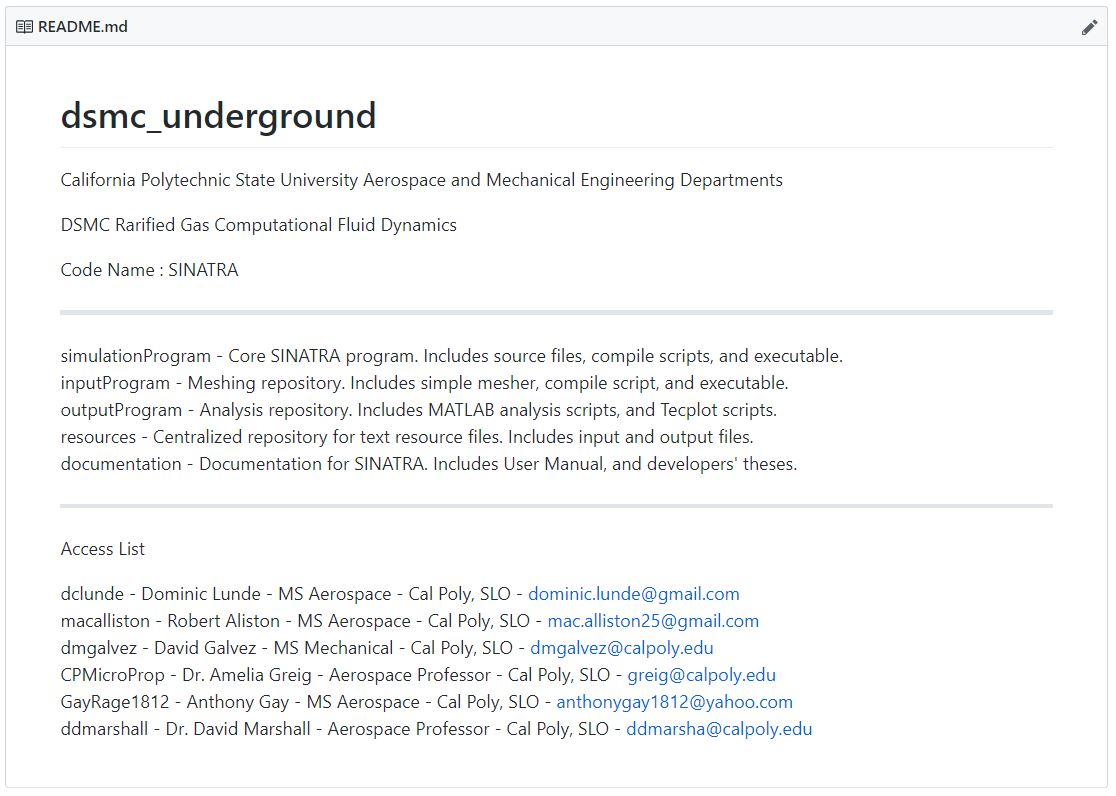
\includegraphics[width=.95\textwidth]{Readme.JPG}
\centering
\caption{SINATRA's main ReadME page}
\label{fig:readme}
\end{figure}


\subsection{Doxygen}
Doxygen is a automatic documentation creator from source code \cite{doxygen}. It was chosen, configured, and used to create the SINATRA Developer Manual. Doxygen is given access to the source code, which it searches through and creates comprehensive documentation of the code base. For SINATRA, it creates descriptions of all of the classes, functions, and files. It shows what each class consists of. For example, it shows that the Mesh class contains structure classes, public types, public member functions and more as seen in figure \ref{fig:Doxygen_Mesh}. It is build in HTML so each attribute is linked to the actual function. It is also possible to see the location of that item in the source code. \par
\indent The important part of Doxygen is that it allows the user to customize the documentation. It allows the HTML file to be built in many different ways to make it work best for SINATRA. But more importantly, it takes comments made in the source code about the attributes and displays them in a clear and concise way. This a developer to quickly find an attribute, where it is referenced in the rest of the source code, where it is built, and what the creator commented about it. This allows new developers to quickly learn SINATRA and start developing their own features. It also allows quick debugging of heritage code by new developers, which ensures that SINATRA will not fall victim to an error that can only be reasonably fixed by the original developer. The author has created a Doxygen manual of SINATRA, as well as a Doxygen input file and batch script for easily updating the manual as more developers add to SINATRA. See Appendix \ref{app:doxygenlists} for a list of all classes and files in SINATRA which have been commented with Doxygen. This is not a comprehensive guide to exactly what each function and variable does, but the author has commented every function in SINATRA to guide new developers. 


\begin{figure}
\includegraphics[width=.95\textwidth]{Doxygen_Mesh.png}
\centering
\caption{Documentation created by Doxygen for the Mesh Class}
\label{fig:Doxygen_Mesh}
\end{figure}


\subsection{User Distribution}
% 
% TO DO Figure out user end documentation

\section{Code Structure}
\subsection{Designed Work Flow}
There are three main sections to a CFD analysis; Meshing, Simulation, and Analysis. DSMC-PIC is a subsection of CFD, therefore the original developers have designed systems for all three sections. However, most  CFD analysis does not require the user to do all three tasks each time. There are many different analysis tasks on the same results from a simulation with a single mesh. There are many different simulations possible with the same mesh. Therefore, SINATRA was broken down into 3 parts according to the three tasks it is able to accomplish. Each of those sections have their own repository, source code, and executables. They also share a resources repository between them. This allows the user to work in the meshing system and create the mesh or meshes necessary for their task. Then they move to the simulation system and use the newly created meshes as part of the simulation input. Once they have simulated the domain, they can take the created output files and run different analysis codes or create their own for their specific task. 


% TO DO make sure that  cart3d has a 3d octree mesher
% TO DO - do I need trademark things here?

\begin{figure}
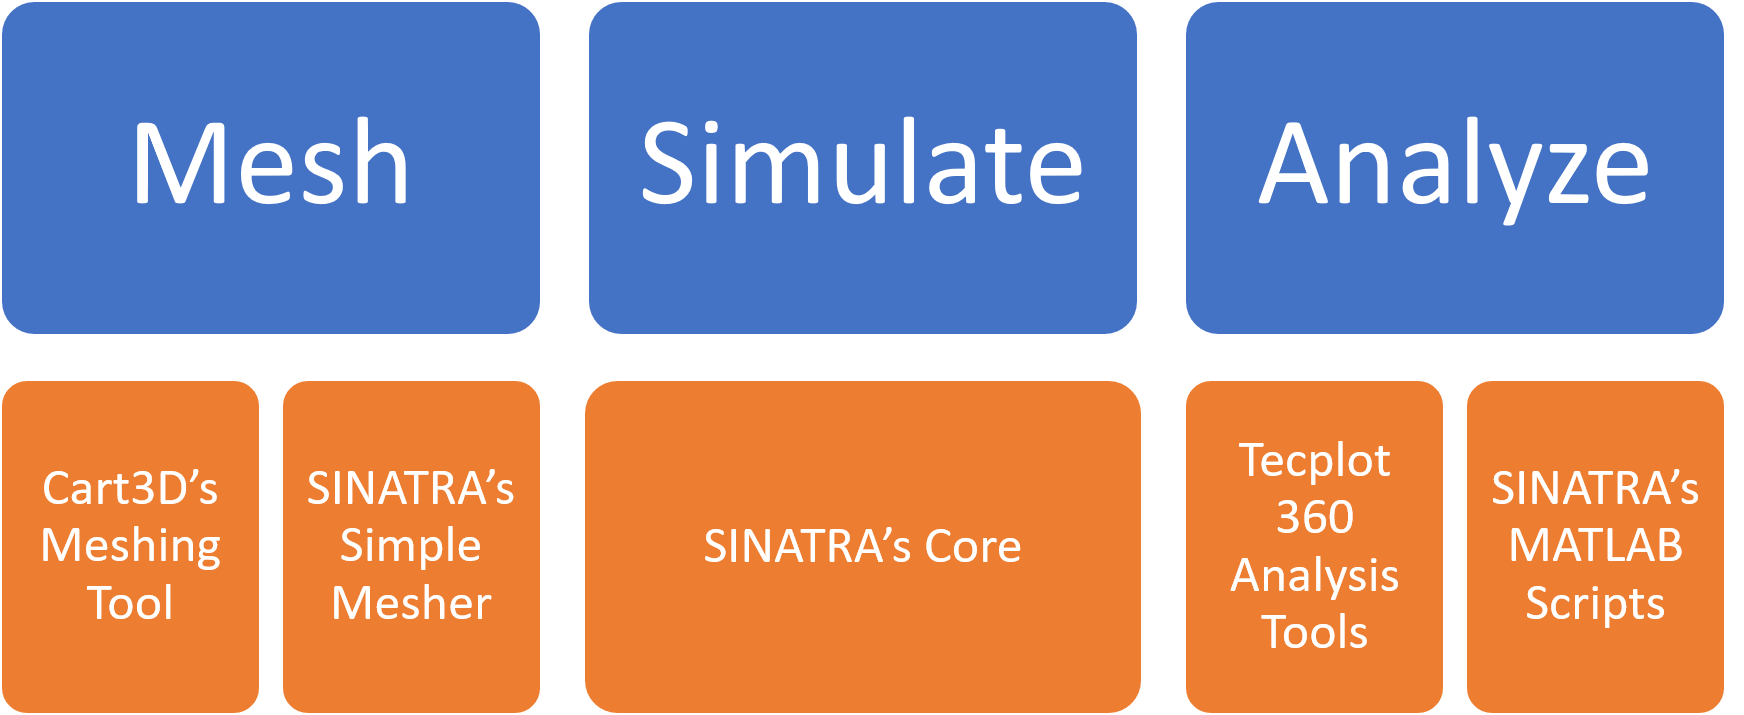
\includegraphics[width=.95\textwidth]{figures/UserWorkFlow.png}
\centering
\caption{Work flow System for SINATRA}
\label{fig:UserWorkFlow}
\end{figure}

\subsection{Mesh}
% TO DO talk about auto meshing and auto timesteps
% TO DO talk about new meshing with objects
The original developers have designed this work flow for SINATRA while including the option for third party software to be used for the meshing and analysis sections. As seen in figure \ref{fig:UserWorkFlow}, Cart3D\textsuperscript{TM} \cite{cart3d} was chosen to be the meshing 3rd party additional tool. Meshing a domain for SINATRA requires an Octree Mesh. For cases where the domain is empty, the homegrown SINATRA meshing tool is quick and simple. However, when an object is added to the domain, meshing becomes a much more complicated task; this is outside the scope and purpose of SINATRA. Cart3D\textsuperscript{TM} is a CFD analysis tool by NASA which is available to universities. It has within it a three-dimensional octree meshing tool which can take geometries and domain sizing as inputs. SINATRA will take the outputted mesh and use it for Simulations. Cart3D has not been tested with SINATRA. It has been slated for future work for another developer to fully integrate Cart3D\textsuperscript{TM} and geometry boundaries with SINATRA\footnote{It may be necessary to run Cart3D within a Linux\textsuperscript{TM} virtual box for Windows\textsuperscript{TM} users}. \par

\subsection{Simulation}

SINATRA has been designed to be simple to develop and execute. Execution is completed through one executable file and one input text file. For simplicity, Windows\textsuperscript{TM} users can drag the .txt file onto the .exe file to run the simulation. SINATRA was deliberately built to be machine independent to reduce the risk of the code not being developer further or used for new tasks. Therefore, the executable and output do not depend on using a specific Integrated Developer Environment like Visual Studio\textsuperscript{TM} or even using a certain operating system. A user can run many simulations or string together meshing, simulating, and analysis simply through a batch script. An example script is shown in Appendix \ref{app:examplescript}. \par
Because SINATRA was built to be platform independent, it is very easy to compile. It requires only a single command with zero libraries.\footnote{Need openmp for parallelization} There are sample compile statements in the ReadME and compile scripts, but even an intermediate C++ coder could figure out how to compile SINATRA from the file list alone. This helps new developers move quickly through the code learning phase and can even allow beginners to explore the code base and test more complicated features. SINATRA has been tested through being compiled with various compilers and on different operating systems.  

% TO DO add compile statements to the readme
% TO DO add ppt graphic of this codeflow one with all the files and titles
% Future - add example of scripting all of them together
% Future - make an input file for meshing

\subsection{Analysis}
% Future make simple tecplot analysis script
% TO dO add citattions of david and macs thesies
% TO DO make analysis functions which gooes through all the cells (send anamynous function)


 After the simulation phase is completed, the user can use the SINATRA output files for analysis. The original developers created MATLAB scripts within SINATRA which do basic types of analysis. For other analysis, Tecplot 360\textsuperscript{TM} \cite{tecplot} has been chosen as a third party tool. Tecplot\textsuperscript{TM} is a specific CFD analysis and visualization tool which can show the mesh, geometry, and fluid flow. It includes robust visualization and animation tools as well as various analysis functions. SINATRA can output data in a format which Tecplot\textsuperscript{TM} reads natively. Tecplot\textsuperscript{TM} and SINATRA's integration has been tested and used by the first developers.\par
 \indent SINATRA's analysis section has not been built with an encompassing set of features to complete any task. It is up to the future users to determine the analysis they need to accomplish, edit SINATRA's output class to accommodate, and compile the output data into the format they need. This can be completed through looking at SINATRA's output class and reformatting other analysis techniques for the task at hand. Tecplot\textsuperscript{TM} and the included MATLAB scripts can do a majority of the the beginning analysis, but the most detailed tools will need to be built by new developers. 


\subsection{Code Flow} % I think this goes somewhere else. another section. maybe beginning of electric
 
 
\subsection{Execution Time} % I think this goes under improvements...
A DSMC code is by nature a very computationally intense program. It requires a large amount of memory to store all of the data of each particle and mesh cell. It requires a lot of computational power to calculate the movement and collisions. Therefore, it is important to design the code to be efficient and powerful. This is why C++ and classes were chosen for SINATRA. However, it is still a slow simulation for a large meshes with high particle densities. It is slated as future work for a developer who specializes in computer science and computational optimization to reduce the execution time of large SINATRA runs. However, there are a few bottlenecks and available improvements which were added by the author. These help manage simulation time, especially when the Poisson equation solver is included.\par
The simplest and most effective way to reduce simulation time on a DSMC simulation is parallelization. Parallelization is a complex and involved field with many competing ideas on best practices. There are many discussions about best ways to parallelize DSMC codes and PIC codes. Parallelization itself is also on the forefront of new technology in this age. Moore's law has allowed programmers to have a large amount of memory for their simulation, so that is rarely the constricting factor. Processors seem to have become as powerful as they will be for user made systems on languages like C++\textsuperscript{TM}. However, breaking the simulation between multiple cores or even within the GPU seems to be the new normal for decreasing execution times. For SINATRA, there are many parallelization possibilities. It is slated for future work for another developer to optimize the parallelization capacity. At this time, simple parallelization has been developed by the author. During the particle propagation phase, there is no interaction between the commands. Therefore, it can be parallelized by using the library openmp\textsuperscript{TM} \cite{openmp}. This can be enabled through an optional keyword in the input file and ensuring the library is included in the compile statement. \par
Another simple process to reduce the execution time is during the linking phase. After the particles are created, they must be associated with the cells that they are in. To do this it requires a double for loop with particles inside cells. This is a very slow process. A few time reduction techniques have been implemented by the author. However, there is a simpler solution. There is an option in SINATRA to seed particles in a uniformly random way \cite{Galvez2018a}. This method creates the same number of particles in each cell but randomly distributes them within the cell. Therefore, this linking process can be removed completely and the execution time reduces significantly. \par
Finally, an important tool for execution time analysis is a profilier. A profilier allows the user to view exactly how often each line of code is run, how long it takes to run, and the subprocesses which contribute to that execution time. This is a strong way to identify simple coding bottlenecks and optimizing the coding time. The author has set up the compiling and code base in order to fit with the profilier Very Sleepy\textsuperscript{TM} \cite{Sleepy}. This is a light and simple profilier which shows each line of the source code and the timing involved. \par


% Add Paralization in the input file
% ADD table of a simulation with each of these items enabled
% Cite processer information
% Cite DSMC paralization papers


\section{User Interfaces}
\subsection{Input Files}
sinatra is not built for error management
\subsection{Graphical User Interface}
The main goal of SINATRA is to be able to simulate rarefied gas for research purposes. It is aimed for use by Faculty, Graduate Students, and specialized Clubs in focused research and projects. However, a DSMC-PIC simulation is a useful tool for even undergraduate classes to test and work with. With that purpose in mind, a Graphical User Interface (GUI) for SINATRA has been created. This GUI is built using MATLAB's Guide tool. It allows a user who has never seen the source code to be able to set up and run simulations. It is built with the expectation that the user does not know how to set up a SINATRA run. \par
The GUI allows the user to input the various parameters of a SINATRA run. It does low level error checking on their input to help the user make simulations without many errors. Then the user can create an input text file through a click of a button. The simulation converts the user's inputs into the format of Sinatra's input file. Then the user can select 'Run' and the GUI will takes a current distribution of SINATRA's executable and run it with the recently created input file.

% Include photo of GUI


\chapter{Charged Particles}
\section{Particle In Cell}
% Making it a charged simluation
% Adding the particle in cell solvers
\subsection{Code Flow}
% How this changes the code flow from before
\subsection{Equations}
\subsection{Finite Volume}
\subsection{Execution time}


\chapter{Future Work}
\section{Future Work}

Because of the nature of SINATRA, it is expected for there to be a large amount of future work. This code base is not a new concept in the world of DSMC and PIC or even DSMC-PIC. The important part about this is that it will be developed further to a point where Cal Poly has a homegrown code which is state of the art and can help develop new Aerospace technology.

\section{Boundaries}

One part of SINATRA which is underdeveloped is the handling of boundaries. Currently, SINATRA handles the main 6 boundaries. It has the capability to define the type of wall and the characteristics of the particles flowing through that wall, but it ignores any boundaries inside of the domain, and the 6 wall faces are all symmetric, it cannot split a wall into multiple types or characteristics. While dealing with boundaries inside the domain will not be needed for a plasma plume, it will be important to be able to split the boundaries so that part of the wall can simulate the thruster nozzle. The path forward for boundaries is twofold. First, a boundary class needs to be build within SINATRA which allows the user to specify sections which will be different from the rest of the domain. At that stage it would be reasonable to simulate a thruster nozzle. \par

\indent The next stage would be to build Cart3D integration. Cart3D is a meshing software that can create an octree mesh which includes internal domain boundaries. This allows a user to import a CAD file and get out a mesh which SINATRA can understand. This is critical for upper atmosphere calculations around aircraft or spacecraft bodies. It can also be used for objects in Low Earth Orbit. The Cart3D tool will allow users to specify what each external and internal boundary type is and can split these boundaries into much smaller pieces. It can also dynamically change the mesh size depending on distance to a wall and other user specifications which will allow for more accurate DSMC-PIC simulation data. This integration will need to be completed before SINATRA can create useful simulation results. \par


\section{Electric Thruster}

As mentioned above, in order for an accurate electric thruster simulation there will need to be changes in how boundaries are handled in SINATRA. This is the most important change that will be needed for accurate simulations of electric thruster plumes. The next important upgrade would be to the Poisson solver. Currently, a finite volume solver is being used. This is a good robust solver which is well researched and understood, but it has a few restrictions. First, and most importantly, it expects the mesh to be evenly sized across the entire domain. This is works with the current version of SINATRA with the home-built meshing software; however, once the boundaries are changed to where the mesh is not completely uniform, the Poisson solver will break. This solver also can only handle straight boundaries, which may be acceptable because the DSMC portion can only handle straight approximations of curves on account of the octree mesh. There are many other options for a Poisson solver which are explored in PIC research. For example, the BLANK solver from BLANK cite{Something} would be a good option for SINATRA. This upgrade would also greatly reduce the execution time, and therefore allow for larger and more accurate simulations. \par


\section{Charged Particles}

There are many faces to simulating charged particles. While the author has captured the largest features of charged particles, there are many other physical attributes which make charged particles a complicated and interesting subject. There are two main physical properties which would be the most likely candidates to be added to SINATRA. They are charged collisions and surface interactions. \par

\indent When charged particles are involved there are many new types of particle collisions. There are ionization and recombination collisions. These are being ignored in SINATRA because the electrons are being modeled as a fluid; however, if magnetic fields were to be included, for example for a magnetic nozzle, or if the grids need to be modeled in SINATRA, then this assumption would no longer be valid. The simulation would have to drastically reduce its simulation time step for the fast electrons and also need to consider ionization and recombination collisions. There are also chemical interactions that are also not being considered in the scope of this project. Both of those types of collisions will most likely not be needed for accurate plasma plume simulations. In order for these collisions to be included as well as the DSMC modeled collision schemes the collision class will need to be updated to be able to handle multiple schemes within the same simulation. \par

\indent However, Charge exchange collisions will need to be eventually included. Charge exchange collisions are instances where a charged ion’s electron cloud will interact with a neutral atom electron field cite{pic}. There is a possibility in these collision for an electron to be stripped from the neutral atom to the charged ion. The charge is exchanged between the two particles; the neutral atom becomes a charged ion and the charged ion becomes a neutral atom, but there is no significant change in momentum. This type of collision is common and significant in electric thruster plumes. While most thrusters are efficient at ionizing the propellant, there are still neutral atoms which come out of the chamber and into the plume. Their relatively slow velocities cause the relative density of the neutral atoms to be high near the thruster nozzle. Charge exchange collisions (CEX) are therefore likely. The resultant slow-moving ions are very susceptible to the radial component of the electric field set up by the plume. While the fast-moving ions will diverge, they do so slowly because of their high initial velocity. however, these new ions are moving slowly and therefore are more easily affected by the radial electric field. They create what is called CEX wings \cite{cex_wings}. These can have large impacts on electric thruster design and therefore need to be added to SINATRA eventually.


\begin{figure}
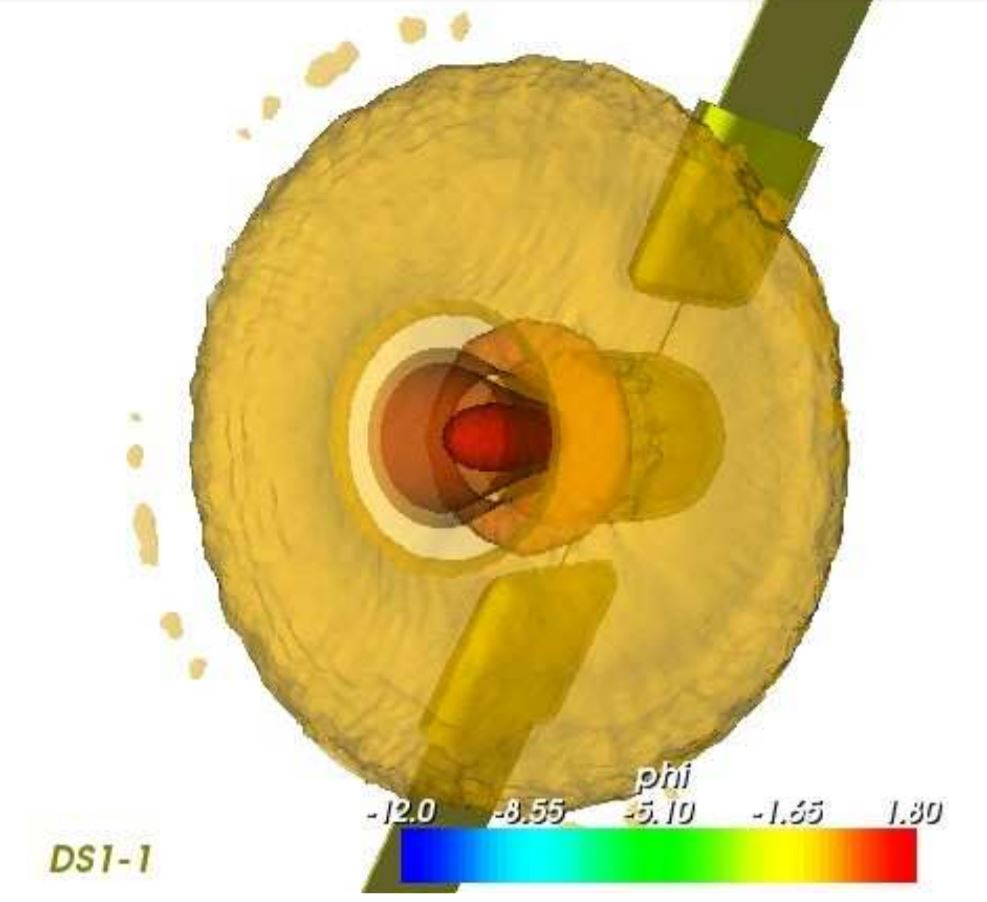
\includegraphics[width=.65\textwidth]{CEX.JPG}
\centering
\caption{Visualization of CEX wings\cite{cex_wings}}
\label{fig:CEX}
\end{figure}

\indent Another important difference from neutral particles that arises when doing a charged particle simulation is surface interactions. SINATRA models various types of surface interactions through its boundary handling. There can be inflow, outflow, specular and diffuse walls. However, especially with CEX collisions, charged particles can interact with a spacecraft surface and impart their charge onto it \cite{surface_charge}. The surface can be modeled as a grounded conductor or as a perfect insulator or as a mix between the two. This type of modeling will need to be included into SINATRA whenever boundaries are introduced into the domain.

\section{SINATRA Efficiency and Capability}

There are many sections in SINATRA that need to be updated before SINATRA can be used as a cutting edge research tool. It was developed by Mechanical and Aerospace engineers, not by computer scientists, therefore, many of the algorithms, storage methods, and memory access are not optimized. The author has removed the largest and simplest bottlenecks, but there are many more areas of optimization. The next largest bottleneck is sampling of data. When SINATRA samples data from the simulation, it prints it out into text files. This printing is one of the slowest portions of the simulation. Tecplot has an API which allows users to print binary files and for Tecplot to read those. This was attempted by the original developers, but they were not successful. It requires a deeper understanding of C++ and binary. There are many examples of this throughout the code which can be optimized by a developer with that type of skill set. \par

\indent Within that similar skill set lies parallelization. Similar to the bottlenecks above the author has implemented a simple version of parallelization, however, there are many better ways to implement it. It could be implemented by splitting the domain into multiple pieces and the octree mesh makes this a viable option. Another option would be to split a larger section of each timestep into many parts. The simulation could also be parallelized by having each core run the same simulation and calculate the time average. Then the multiple different simulations could be averaged as a way to reduce the randomness of DSMC so that an accurate solution is calculated. Parallelization is still on the cutting edge of computer science, and therefore this would be a fruitful project for a developer with experience in this area. \par

\indent Within the DSMC community, there are many schools of thought about the best way to work with time steps and mesh sizes citeBird. It is possible to have variable time steps as well as variable mesh sizes. It is also possible for the time step to change for each particle depending on their velocity and the size of the mesh cell they are within. There are algorithms which create a mesh which changes size depending on the average number of particles in a cell. This creates a mesh which changes with the flow and eventually sets up an optimal mesh for that simulation and steady state flow condition. SINATRA is a currently at its first iteration, therefore it uses a fixed time step for all particles and a fixed mesh. Upgrading SINATRA to a more complicated time step and mesh algorithm would be a good project for a future developer. In order to keep charged particle capability, the Poisson solver would have to be upgraded at the same time because it is currently based on the fixed mesh. This upgrade could greatly reduce SINATRA’s execution time and, therefore, allow higher resolution and accurate simulations. \par

\section{Systems Operations}

It will be important to continually update the systems engineering sections of SINATRA. The author has set up systems which will hopefully be helpful at keeping SINATRA up to date and relevant, but they will need to be monitored and maintained
 \par

\indent First, the simple distributions need to be kept up to date. There are distributions for Windows, Linux, and Mac. If SINATRA continues to grow at Cal Poly, an official release website with version control can be set up. Until then it will be released through .zip files being sent to the new users, therefore, the distributions need to be up to date with the current stable version of SINATRA, input files, and GUI. \par

\indent The GUI will also need to be updated as there are changes to the input class. Whenever the input class requires a different way to input variables to the simulation, the GUI will also need to be changed to accommodate for that. It will also have to be updated when the interface changes for boundaries and output options. It is not difficult maintenance the GUI, but it can easily become obsolete if it is left alone while developing. \par

\indent The author has ensured that the Github repository is kept up to date and clean as much as possible. It will be necessary to use the Github while developing new code. It can be easy for new developers to develop in their own local machine and ignore the Github. This ruins the continuity of the version control of Github and more importantly makes it harder for new developers to add their contribution. The Github should be kept as a version of the code which can be easily shared with new developers and they will not be confused, nor distracted by extra files and information. If SINATRA is well taken care of, it will become a legacy code that will allow Cal Poly to shine as a school with advanced modeling skills and allow new and revolutionary technology to come from ’Learning by Doing’.






\nocite{*}
\bibliography{bibliography}

% Indents Appendix in Table of Contents
\makeatletter
\addtocontents{toc}{\let\protect\l@chapter\protect\l@section}
\makeatother

% Hack to make Appendices to appear in Table of Contents
\addtocontents{toc}{%
   \noindent APPENDICES
}
\begin{appendices}
\chapter{Example Batch Script}
\label{app:examplescript}
Seen below is an example batch script written for Windows\textsuperscript{TM}. 
\chapter{Doxygen Class and File Lists}
\label{app:doxygenlists}


\textbf{Classes}
\begin{figure}[h]
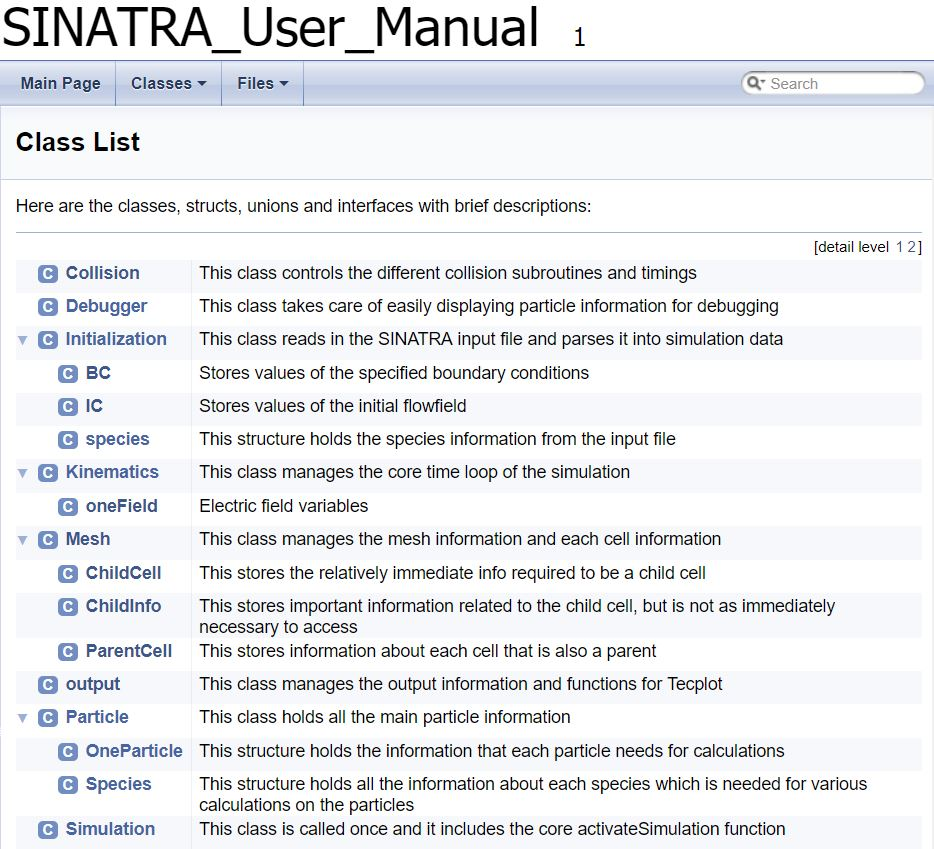
\includegraphics[width=.95\textwidth]{figures/ClassList.JPG}
\centering
\caption{List of all Classes commented through Doxygen}
\label{fig:ClassList}
\end{figure}


\newpage
\textbf{Files}
\begin{figure}[h]
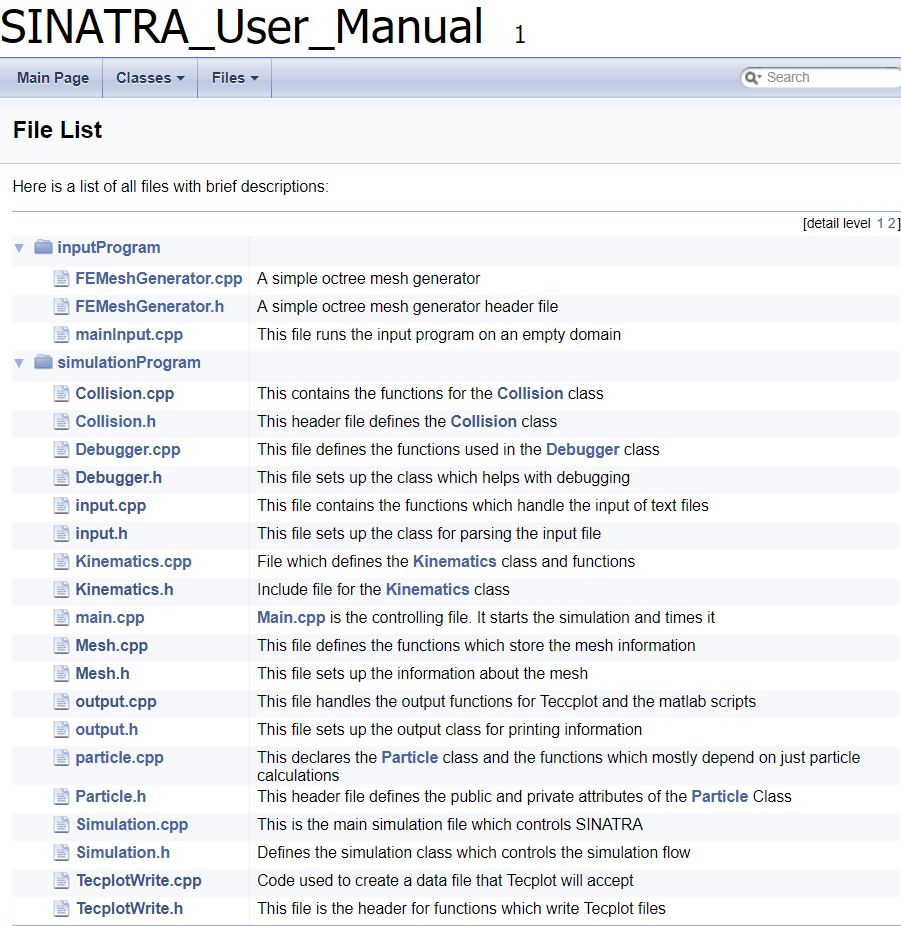
\includegraphics[width=.95\textwidth]{figures/FileList.JPG}
\centering
\caption{List of all Files commented through Doxygen}
\label{fig:FileList}
\end{figure}



\chapter{Simple Distribution Walkthrough}
\label{app:walkthrough}
Seen below is a simple tutorial for starting with SINATRA. It can be found in the documentation/SimpleDistribution directory as ReadMe.md within each specific OS's directory.

\begin{verbatim}
SINATRA Simple Distribution Manual
Dominic Lunde


Hello! Welcome to a tutorial on how to use SINATRA.

First, requirements
1) Windows OS
2) Matlab or Matlab runtime - for output only

This will walk you through a simple simulation case. 
Then it will show you how to use the GUI and then you can have fun!



Step 1 - Mesh

We must create a mesh file. This is done through
 the Mesh.exe executable.
The MeshInput.txt file is already set up to create
 8 cells through 1 cut.
 
Therefore we can run the mesher by either:
a) Dragging MeshInput.txt onto Mesh.exe
b) Running "Mesh MeshInput.txt" into a
 command window set to this directory

After this is done, you should see your
 mesh file as a .plt file appear. Good!


Step 2 - Simulate

Now we can simulate some particles. 
Complex_Input.txt is set up to use
 8 cells and run 10 timesteps

Therefore we can run the mesher by either:
a) Dragging Complex_Input.txt onto DSMC.exe
b) Running "DSMC Complex_Input.txt"
 into a command window

All done! You will see a file called SINATRA_OUTPUT.txt.
This shows you very simple time step info. 
You will also see SINATRA_uniform_properties_000001.plt.
This has Tecplot data from the first time step.


Step 3 - Analysis

We want to see those particles move right? 
We need to change some things first.
Open Complex_Input.txt and go
 to the "Output Information" Section
Between the Tecplot Sample Frequency and the *** add this.

Particle Animation
0
1
VelocityOutput\velocityFromParticles_

The first line is the trigger word, next is the start time,
 then the frequency of output, and finally the base filename.
--Create the folder VelocityOutput 
 so these files have a place to go. 
Now run the simulation again. 

Now if you open VelocityOutput you will see 11 files! 
We can use those to view the particles and their movements.
--Open FlowVelocityDistributionAnim.m in Matlab and run

A file called SINATRA_gif.gif will be
 created and you can see your particles!
However, it's a mess and they don't seem to move. Let's change that. 
In Complex_Input 
--Change the Time Step to 1e-5 
--Change the Total Simulation Time to 10e-5.
This will allow the particles to move further each frame. 
Now let's make less particles.
--Set the Number Density to 1e-22.
Now rerun the simlulation and analysis
 and boom! Particles in a box. 

Step 4 - GUI

Now I'm going to let you play with the GUI. Open up SINATRA_GUI.exe. 
We're going to have to change a few things. 
SINATRA Output file - SINATRA_OUTPUT.txt
Tecplot Output      - SINATRA_uniform_properties.plt
Velocity Output     - VelocityOutput/velocityFromParticles_
Mesh File           - FE_NodeLocations_UnitCubeQuad8Cells_TEC.plt
Input File          - Complex_Input.txt

This GUI prints input files. 
Try it by pressing "Write File" then "Open File". 
Then change something and see how it changes the input file. 
Finally, you can press "Simulate" to run that input file on DSMC.exe.

Have fun!


\end{verbatim}
\chapter{Input File Guide}
\label{app:inputfileguide}
This is the Input File Guide. It can be found in the ReadMe for the resources file. It explains each command of the input file and how it works.

\begin{verbatim}
Input file Guide  
  
SINATRA reads input files line by line.   
It searches for key words and ignores words which don't fit them.   
Then it takes the items in the line under the keyword and
 parses that for the simulation.  
  
There are 6 sections to the input file. The sections are
 deliminated by *  
After the first section, the order of the sections does not matter.  
The order of the trigger words do not matter within the sections  
  
Section 1 - This is the intro section. It does not have
 a header trigger  
  
"Mesh Input Filename"                               - path name to 
 the file which holds the mesh information  
"Number of Real Particles to Simulation Particles"  - number as a 
 double which is the ratio of real particles per simulation particles  
"Boundary Conditions"                               - boundary
 conditions of the walls. 6 space deliminated string arguments
  for the type of the walls. Options are "INFLOW","OUTFLOW",
   "SWALL","DWALL","PWALL". Order of the walls is
    -X,+X,-Y,+Y,-Z,+Z.  
"Collision Scheme"                                  - an integer
 which signifies which collision scheme to use  
"Sphere Model"                                      - an integer
 which signifies which sphere model to use  
"Total Simulation Time"                             - a double
 showing the total time the simulation should run  
"Time Step"                                         - a double of
 the amount of time for each time step  
  
  
Section 2 - Trigger "Initial Conditions"   
This section contains simple initial conditions  
  
"Number Density"     - a double with the number density
 for the whole simulation  
"Mixture"            - a space separated line of alternating
 integers and doubles. The first number is the species
  id and the second is the percentage it is in the
   mixture being simulated  
"Stream Temperature" - a double temperature in Kelvin  
"Stream Velocity"    - space separated doubles which are 
 the X,Y,Z direction of the stream velocity  
  
  
Section 3 - Trigger "Boundary Condition Information"  
This section contains the information about the Boundaries  
  
There are 6 items which should be put in this. 
 They each start with "BC X".   
X is the number of the boundary from 0 to 5
 following -X,+X,-Y,+Y,-Z,+Z.   
Each section ends with a "&".   
They contain  
  
"Number Density"  
"Mixture"  
"Stream Temperature"  
"Stream Velocity"  
  
where each are defined the same way as in Section 2.  
  
  
Section 4 - Trigger "Output Information"  
This section defined the output variables needed to view the data  
  
"Output File Name"           - a string path to
 where the simple output file will be placed  
"Tecplot Base Name"          - a string path which
 is the base of the Tecplot output files. It will be
  edited with timestep information for each new file.
   WARNING - if the folder path does not exist, no
    files will be created.  
"Sample Cell Type"           - a flag for which sampling 
 should be used. 1 stands for leaf cells and 2 stands for 
  the immediate parents of the leaf cells  
"Tecplot Sample Frequency"   - an integer of the number of
 time steps between each sampling  
"Tecplot Sample Start Time"  - a double which defines the
 start time for Tecplot sampling  
"Particle Animation"         - a three lined argument.
 first is start time. second is frequency (integer), and
  final is the base file name for the animation files  
  
  
  
Section 5 - Trigger "Species Information"  
This section holds the information for the species to be used  
  
Each species section starts with the trigger "Species"  
After this a list of items are included which are added
 to that species class  
These are listed below in order.   
  
Reference Temperature            - Kelvin    - double  
Molecular Diameter               - meters    - double  
Mass                             - kilograms - double  
Rotational Degrees of Freedom    - number    - integer  
Vibrational Degrees of Freedom   - number    - integer  
Characteristic Temperature (Rot) - Kelvin    - double  
Characteristic Temperature (Vib) - Kelvin    - double  
Viscosity Index                  - number    - double  
Viscosity Coefficient            - number    - double  
Charge                           - Columbs   - double  
VSS Exponent (VSS sphere only)   - number    - double    
  
  
Section 6 - Trigger "Optional Keywords"  
Optional items for the simulation.   
These don't necessarily have a second line, they can be
 used just as single line triggers  
  
"diffusion"              - if trigger is there, enables 
 the diffusion test case  
"init_velocity_gradient" - Next line is the direction of 
 the gradient (X,Y,Z). Next line is 6 item deliminated by
  spaces with the inputs for the velocity gradient in the
   normal 6 direction order  
"Charged Simulation"     - triggers a charged simulation  
"Parallel Enabled"       - triggers a parallel simulation   
  
  
Any other questions about the input file can be solved
 by emailing the original developers. Or by reading 
  through input.cpp and input.h.  
  
\end{verbatim}
\chapter{SINATRA Input Files for Validation}
\label{app:validation_input}

\textbf{8 Cell Convergence Visual}

\begin{verbatim}
    *** SINATRA Input File ***
*** Created by User domin with SINATRA_GUI.m ***
*** 09-May-2019 12:23:24 ***

Mesh Input Filename
../resources/FE_NodeLocations_UnitCubeQuad8Cells_TEC.plt

Number of Real Particles to Simulation Particles
1e+19

Boundary Conditions
OUTFLOW DWALL DWALL DWALL DWALL DWALL

Collision Scheme
0

Sphere Model
1

Total Simulation Time
1e-08

Time Step
1e-08

Initial Conditions

Number Density
8e+19

Mixture
1 1.0

Stream Temperature
300

Stream Velocity
0 0 0

***

Boundary Condition Information

BC 0

Number Density
1e+23

Mixture
1 1

Stream Temperature
300

Stream Velocity
0 0 0

&

BC 1

Number Density
1e+23

Mixture
1 1

Stream Temperature
300

Stream Velocity
0 0 0

&

BC 2

Number Density
1e+23

Mixture
1 1

Stream Temperature
300

Stream Velocity
0 0 0

&

BC 3

Number Density
1e+23

Mixture
1 1

Stream Temperature
300

Stream Velocity
0 0 0

&

BC 4

Number Density
1e+23

Mixture
1 1

Stream Temperature
300

Stream Velocity
0 0 0

&

BC 5

Number Density
1e+23

Mixture
1 1

Stream Temperature
300

Stream Velocity
0 0 0

***

Output Information

Output File Name
../resources/SINATRA_OUTPUT.txt

Tecplot Base Name
../resources/TecplotOutput/SINATRA_uniform_properties.plt

Sample Cell Type
1

Tecplot Sample Frequency
10

***

Species Information

Species 1 (Nitrogen, N2)
273
4.17e-010
4.65e-026
2
2
2.88
3371
0.74
1.656e-05
1e-19

Species 2 (Oxygen, O2)
273
4.07e-010
5.31e-026
2
2
2.07
2256
0.77
1.919e-05
0

Species 3 (Argon, Ar)
273
4.17e-010
6.63e-026
0
0
0
0
0.81
2.117e-05
0

Species 4 (Carbon Dioxide, CO2)
273
5.62e-010
7.31e-026
3
4
0.561
1700
0.93
1.380e-05
0

***

Optional Keywords

Charged Simulation

***

\end{verbatim}

\newpage

\textbf{4096 Cell Convergence Visual}

\begin{verbatim}
    *** SINATRA Input File ***
*** Created by User domin with SINATRA_GUI.m ***
*** 09-May-2019 12:23:24 ***

Mesh Input Filename
../resources/FE_NodeLocations_UnitCubeQuad4096Cells_TEC.plt

Number of Real Particles to Simulation Particles
1e+19

Boundary Conditions
DWALL DWALL DWALL DWALL DWALL DWALL

Collision Scheme
0

Sphere Model
1

Total Simulation Time
1e-08

Time Step
1e-08

Initial Conditions

Number Density
1e+24

Mixture
1 1.0

Stream Temperature
300

Stream Velocity
0 0 0

***

Boundary Condition Information

BC 0

Number Density
1e+23

Mixture
1 1

Stream Temperature
300

Stream Velocity
0 0 0

&

BC 1

Number Density
1e+23

Mixture
1 1

Stream Temperature
300

Stream Velocity
0 0 0

&

BC 2

Number Density
1e+23

Mixture
1 1

Stream Temperature
300

Stream Velocity
0 0 0

&

BC 3

Number Density
1e+23

Mixture
1 1

Stream Temperature
300

Stream Velocity
0 0 0

&

BC 4

Number Density
1e+23

Mixture
1 1

Stream Temperature
300

Stream Velocity
0 0 0

&

BC 5

Number Density
1e+23

Mixture
1 1

Stream Temperature
300

Stream Velocity
0 0 0

***

Output Information

Output File Name
../resources/SINATRA_OUTPUT.txt

Tecplot Base Name
../resources/TecplotOutput/SINATRA_uniform_properties.plt

Sample Cell Type
1

Tecplot Sample Frequency
10

***

Species Information

Species 1 (Nitrogen, N2)
273
4.17e-010
4.65e-026
2
2
2.88
3371
0.74
1.656e-05
1e-19

Species 2 (Oxygen, O2)
273
4.07e-010
5.31e-026
2
2
2.07
2256
0.77
1.919e-05
0

Species 3 (Argon, Ar)
273
4.17e-010
6.63e-026
0
0
0
0
0.81
2.117e-05
0

Species 4 (Carbon Dioxide, CO2)
273
5.62e-010
7.31e-026
3
4
0.561
1700
0.93
1.380e-05
0

***

Optional Keywords

Charged Simulation

***

\end{verbatim}


\end{appendices}

\end{document}
